% Options for packages loaded elsewhere
\PassOptionsToPackage{unicode}{hyperref}
\PassOptionsToPackage{hyphens}{url}
%
\documentclass[
  ignorenonframetext,
]{beamer}
\usepackage{pgfpages}
\setbeamertemplate{caption}[numbered]
\setbeamertemplate{caption label separator}{: }
\setbeamercolor{caption name}{fg=normal text.fg}
\beamertemplatenavigationsymbolsempty
% Prevent slide breaks in the middle of a paragraph
\widowpenalties 1 10000
\raggedbottom
\setbeamertemplate{part page}{
  \centering
  \begin{beamercolorbox}[sep=16pt,center]{part title}
    \usebeamerfont{part title}\insertpart\par
  \end{beamercolorbox}
}
\setbeamertemplate{section page}{
  \centering
  \begin{beamercolorbox}[sep=12pt,center]{part title}
    \usebeamerfont{section title}\insertsection\par
  \end{beamercolorbox}
}
\setbeamertemplate{subsection page}{
  \centering
  \begin{beamercolorbox}[sep=8pt,center]{part title}
    \usebeamerfont{subsection title}\insertsubsection\par
  \end{beamercolorbox}
}
\AtBeginPart{
  \frame{\partpage}
}
\AtBeginSection{
  \ifbibliography
  \else
    \frame{\sectionpage}
  \fi
}
\AtBeginSubsection{
  \frame{\subsectionpage}
}
\usepackage{amsmath,amssymb}
\usepackage{iftex}
\ifPDFTeX
  \usepackage[T1]{fontenc}
  \usepackage[utf8]{inputenc}
  \usepackage{textcomp} % provide euro and other symbols
\else % if luatex or xetex
  \usepackage{unicode-math} % this also loads fontspec
  \defaultfontfeatures{Scale=MatchLowercase}
  \defaultfontfeatures[\rmfamily]{Ligatures=TeX,Scale=1}
\fi
\usepackage{lmodern}
\usetheme[]{Madrid}
\ifPDFTeX\else
  % xetex/luatex font selection
\fi
% Use upquote if available, for straight quotes in verbatim environments
\IfFileExists{upquote.sty}{\usepackage{upquote}}{}
\IfFileExists{microtype.sty}{% use microtype if available
  \usepackage[]{microtype}
  \UseMicrotypeSet[protrusion]{basicmath} % disable protrusion for tt fonts
}{}
\makeatletter
\@ifundefined{KOMAClassName}{% if non-KOMA class
  \IfFileExists{parskip.sty}{%
    \usepackage{parskip}
  }{% else
    \setlength{\parindent}{0pt}
    \setlength{\parskip}{6pt plus 2pt minus 1pt}}
}{% if KOMA class
  \KOMAoptions{parskip=half}}
\makeatother
\usepackage{xcolor}
\newif\ifbibliography
\usepackage{color}
\usepackage{fancyvrb}
\newcommand{\VerbBar}{|}
\newcommand{\VERB}{\Verb[commandchars=\\\{\}]}
\DefineVerbatimEnvironment{Highlighting}{Verbatim}{commandchars=\\\{\}}
% Add ',fontsize=\small' for more characters per line
\usepackage{framed}
\definecolor{shadecolor}{RGB}{248,248,248}
\newenvironment{Shaded}{\begin{snugshade}}{\end{snugshade}}
\newcommand{\AlertTok}[1]{\textcolor[rgb]{0.94,0.16,0.16}{#1}}
\newcommand{\AnnotationTok}[1]{\textcolor[rgb]{0.56,0.35,0.01}{\textbf{\textit{#1}}}}
\newcommand{\AttributeTok}[1]{\textcolor[rgb]{0.13,0.29,0.53}{#1}}
\newcommand{\BaseNTok}[1]{\textcolor[rgb]{0.00,0.00,0.81}{#1}}
\newcommand{\BuiltInTok}[1]{#1}
\newcommand{\CharTok}[1]{\textcolor[rgb]{0.31,0.60,0.02}{#1}}
\newcommand{\CommentTok}[1]{\textcolor[rgb]{0.56,0.35,0.01}{\textit{#1}}}
\newcommand{\CommentVarTok}[1]{\textcolor[rgb]{0.56,0.35,0.01}{\textbf{\textit{#1}}}}
\newcommand{\ConstantTok}[1]{\textcolor[rgb]{0.56,0.35,0.01}{#1}}
\newcommand{\ControlFlowTok}[1]{\textcolor[rgb]{0.13,0.29,0.53}{\textbf{#1}}}
\newcommand{\DataTypeTok}[1]{\textcolor[rgb]{0.13,0.29,0.53}{#1}}
\newcommand{\DecValTok}[1]{\textcolor[rgb]{0.00,0.00,0.81}{#1}}
\newcommand{\DocumentationTok}[1]{\textcolor[rgb]{0.56,0.35,0.01}{\textbf{\textit{#1}}}}
\newcommand{\ErrorTok}[1]{\textcolor[rgb]{0.64,0.00,0.00}{\textbf{#1}}}
\newcommand{\ExtensionTok}[1]{#1}
\newcommand{\FloatTok}[1]{\textcolor[rgb]{0.00,0.00,0.81}{#1}}
\newcommand{\FunctionTok}[1]{\textcolor[rgb]{0.13,0.29,0.53}{\textbf{#1}}}
\newcommand{\ImportTok}[1]{#1}
\newcommand{\InformationTok}[1]{\textcolor[rgb]{0.56,0.35,0.01}{\textbf{\textit{#1}}}}
\newcommand{\KeywordTok}[1]{\textcolor[rgb]{0.13,0.29,0.53}{\textbf{#1}}}
\newcommand{\NormalTok}[1]{#1}
\newcommand{\OperatorTok}[1]{\textcolor[rgb]{0.81,0.36,0.00}{\textbf{#1}}}
\newcommand{\OtherTok}[1]{\textcolor[rgb]{0.56,0.35,0.01}{#1}}
\newcommand{\PreprocessorTok}[1]{\textcolor[rgb]{0.56,0.35,0.01}{\textit{#1}}}
\newcommand{\RegionMarkerTok}[1]{#1}
\newcommand{\SpecialCharTok}[1]{\textcolor[rgb]{0.81,0.36,0.00}{\textbf{#1}}}
\newcommand{\SpecialStringTok}[1]{\textcolor[rgb]{0.31,0.60,0.02}{#1}}
\newcommand{\StringTok}[1]{\textcolor[rgb]{0.31,0.60,0.02}{#1}}
\newcommand{\VariableTok}[1]{\textcolor[rgb]{0.00,0.00,0.00}{#1}}
\newcommand{\VerbatimStringTok}[1]{\textcolor[rgb]{0.31,0.60,0.02}{#1}}
\newcommand{\WarningTok}[1]{\textcolor[rgb]{0.56,0.35,0.01}{\textbf{\textit{#1}}}}
\usepackage{graphicx}
\makeatletter
\def\maxwidth{\ifdim\Gin@nat@width>\linewidth\linewidth\else\Gin@nat@width\fi}
\def\maxheight{\ifdim\Gin@nat@height>\textheight\textheight\else\Gin@nat@height\fi}
\makeatother
% Scale images if necessary, so that they will not overflow the page
% margins by default, and it is still possible to overwrite the defaults
% using explicit options in \includegraphics[width, height, ...]{}
\setkeys{Gin}{width=\maxwidth,height=\maxheight,keepaspectratio}
% Set default figure placement to htbp
\makeatletter
\def\fps@figure{htbp}
\makeatother
\setlength{\emergencystretch}{3em} % prevent overfull lines
\providecommand{\tightlist}{%
  \setlength{\itemsep}{0pt}\setlength{\parskip}{0pt}}
\setcounter{secnumdepth}{-\maxdimen} % remove section numbering
\logo{
\includegraphics[height=1cm,width=3cm]{logo.png}}
\usetheme{Madrid}
\usefonttheme{serif}
\setbeamertemplate{navigation symbols}{}
\usepackage{lmodern}  % for bold teletype font
\usepackage{amsmath}  % for \hookrightarrow
\usepackage{xcolor}   % for \textcolor


\ifLuaTeX
  \usepackage{selnolig}  % disable illegal ligatures
\fi
\IfFileExists{bookmark.sty}{\usepackage{bookmark}}{\usepackage{hyperref}}
\IfFileExists{xurl.sty}{\usepackage{xurl}}{} % add URL line breaks if available
\urlstyle{same}
\hypersetup{
  pdftitle={Leksioni 7},
  pdfauthor={Endri Raco},
  hidelinks,
  pdfcreator={LaTeX via pandoc}}

\title{Leksioni 7}
\author{Endri Raco}
\date{05 May, 2024}

\begin{document}
\frame{\titlepage}

\begin{frame}[allowframebreaks]
  \tableofcontents[hideallsubsections]
\end{frame}
\hypertarget{tuxeb-dhuxebnat-raster}{%
\section{Të dhënat Raster}\label{tuxeb-dhuxebnat-raster}}

\begin{frame}{Të dhënat Raster}
\protect\hypertarget{tuxeb-dhuxebnat-raster-1}{}
\begin{itemize}
\tightlist
\item
  Të dhënat raster përfaqësojnë samples nga fusha (\textbf{fields}) të
  vazhdueshme, të tilla si temperatura, dendësia e gazit, dendësia e
  bimësisë, etj.
\end{itemize}
\end{frame}

\begin{frame}{Të dhënat Raster}
\protect\hypertarget{tuxeb-dhuxebnat-raster-2}{}
Një dataset raster zakonisht është një matricë me dy përmasa:

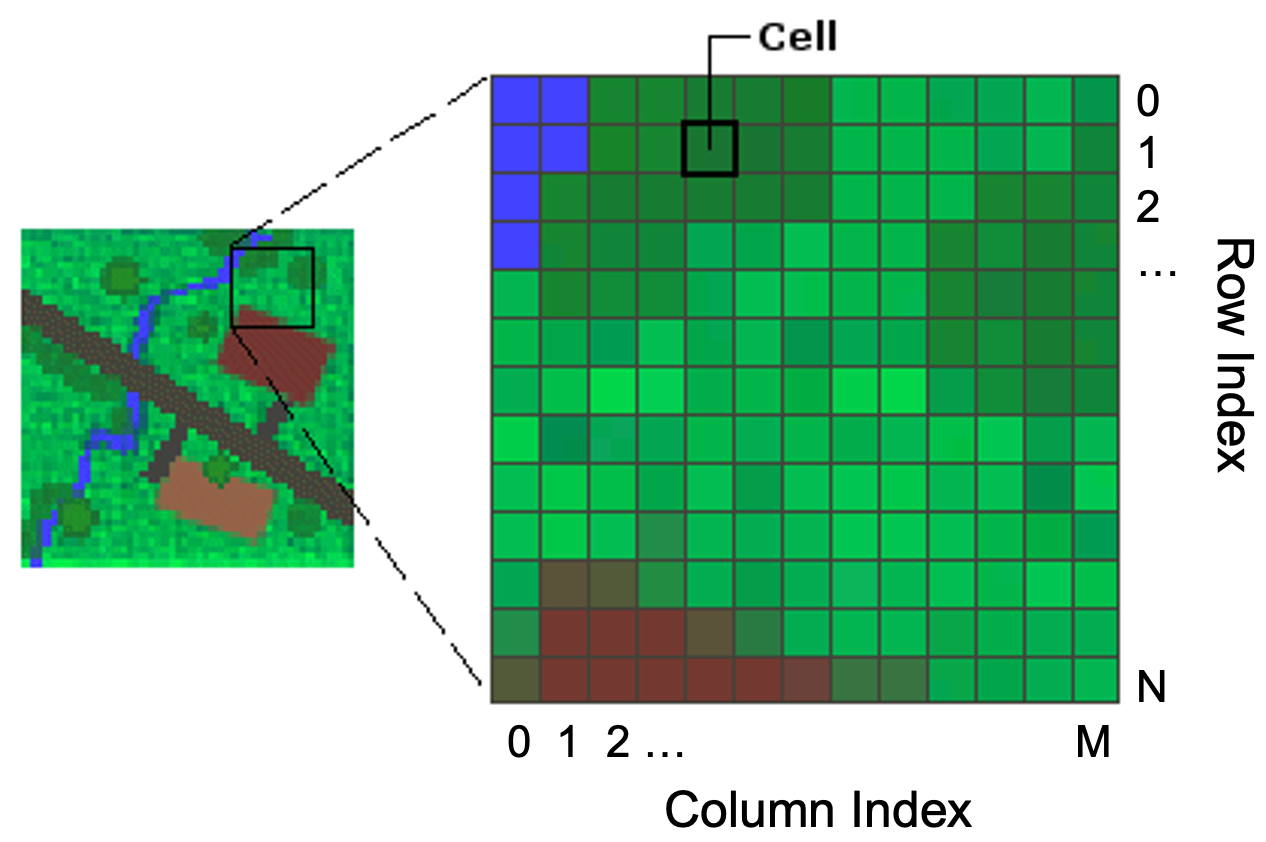
\includegraphics{./Figs/raster_matrix1.png}
\end{frame}

\begin{frame}{Të dhënat Raster}
\protect\hypertarget{tuxeb-dhuxebnat-raster-3}{}
\begin{itemize}
\item
  Një qelizë raster mund të referohet me një indeks dy-dimensional, duke
  treguar një çift \textless rresht, kolonë\textgreater. Këta indekse
  fillojnë nga 0.
\item
  Çdo vendndodhje e indeksit mund të shoqërohet me një vendndodhje
  gjeografike (për shembull, qeliza \textless12,796\textgreater{} mund
  të korrespondojë me lon/lat \textless-0.34521,51.354656\textgreater).
\end{itemize}
\end{frame}

\begin{frame}{Të dhënat Raster}
\protect\hypertarget{tuxeb-dhuxebnat-raster-4}{}
\begin{itemize}
\tightlist
\item
  Kur punojmë me të dhëna raster, shpesh kalojmë nga indeksi raster te
  vendndodhjet gjeografike dhe anasjelltas.
\end{itemize}
\end{frame}

\begin{frame}{Të dhënat Raster}
\protect\hypertarget{tuxeb-dhuxebnat-raster-5}{}
\begin{itemize}
\item
  Nëse një dataset raster përmban më shumë se një matricë, ne i
  referohemi matricave të ndryshme si banda (\textbf{bands})
\item
  Bandat numërohen nga 1.
\end{itemize}
\end{frame}

\begin{frame}{Të dhënat Raster}
\protect\hypertarget{tuxeb-dhuxebnat-raster-6}{}
\begin{itemize}
\tightlist
\item
  Për shembull, një raster i prodhuar nga një satelit mund të përmbajë 3
  banda që përfaqësojnë intensitetin e kuqes, jeshiles dhe blusë.
\end{itemize}
\end{frame}

\begin{frame}{Paketat Python për të dhënat raster}
\protect\hypertarget{paketat-python-puxebr-tuxeb-dhuxebnat-raster}{}
\begin{itemize}
\item
  Python nuk ka një paketë standarde të vetme që ofron të gjithë
  funksionalitetin për të punuar me të dhëna raster.
\item
  Siç është shpesh rasti, në Python ne përdorim një kombinim të paketave
  shumë të specializuara për të arritur një qëllim.
\end{itemize}
\end{frame}

\begin{frame}{Të dhënat Raster}
\protect\hypertarget{tuxeb-dhuxebnat-raster-7}{}
\begin{itemize}
\item
  \textbf{rasterio}: kjo paketë mund të lexojë dhe shkruajë të dhëna
  raster (\url{https://rasterio.readthedocs.io}).
\item
  \textbf{rasterstats}: kjo paketë ofron funksionalitet për statistikat
  zonale (\url{https://pythonhosted.org/rasterstats}).
\item
  \textbf{gdal}: shumë librari në Python (dhe gjuhë të tjera) mbështeten
  në këtë bibliotekë të vjetër, por të qëndrueshme, që ofron qindra
  funksione gjeohapësinore, duke përfshirë përpunimin vektorial dhe
  raster (\url{https://gdal.org}).
\item
  \textbf{numpy}: kjo paketë suporton operacionet e shpejta në matricat
  numerike që janë thelbi i përpunimit gjeohapësinor të rasterit.
\end{itemize}
\end{frame}

\begin{frame}{Shkarkimi i skedarëve nga web-i}
\protect\hypertarget{shkarkimi-i-skedaruxebve-nga-web-i}{}
\begin{itemize}
\tightlist
\item
  Deri tani ne kemi punar me skedare lokalë, por gjithashtu të
  shkarkojmë skedarë nga web-i.
\end{itemize}
\end{frame}

\begin{frame}{Shkarkimi i skedarëve nga web-i}
\protect\hypertarget{shkarkimi-i-skedaruxebve-nga-web-i-1}{}
\begin{itemize}
\item
  Shpesh, setet e mëdha të dhënave ndahen në copa më të vogla dhe
  shkarkimi i tyre manualisht mund të marrë shumë kohë.
\item
  Ky funksionalitet gjithashtu mund të përdoret në script dhe për të
  marrë rezultatet automatikisht.
\end{itemize}
\end{frame}

\begin{frame}{Shkarkimi i skedarëve nga web-i}
\protect\hypertarget{shkarkimi-i-skedaruxebve-nga-web-i-2}{}
Në këtë shembull, do të shkarkojmë skedarë nga një depo GitHub, duke
shkarkuar një skedar raster me paketën.
\end{frame}

\begin{frame}[fragile]{Shkarkimi i skedarëve nga web-i}
\protect\hypertarget{shkarkimi-i-skedaruxebve-nga-web-i-3}{}
\AddToHookNext{env/Highlighting/begin}{\scriptsize}

\begin{Shaded}
\begin{Highlighting}[]
\ImportTok{import}\NormalTok{ urllib.request}

\CommentTok{\# URL to download from}
\NormalTok{url }\OperatorTok{=} \StringTok{\textquotesingle{}https://github.com/endri81/instatgis/blob/master/data/gis3/eu{-}2016{-}nox\_avg.tif?raw=true\textquotesingle{}}

\CommentTok{\# Local file name where the file will be saved}
\NormalTok{file\_name }\OperatorTok{=} \StringTok{\textquotesingle{}data/eu{-}2016{-}nox\_avg.tif\textquotesingle{}}

\CommentTok{\# Download the file}
\NormalTok{urllib.request.urlretrieve(url, file\_name)}

\BuiltInTok{print}\NormalTok{(}\SpecialStringTok{f"Downloaded }\SpecialCharTok{\{}\NormalTok{file\_name}\SpecialCharTok{\}}\SpecialStringTok{"}\NormalTok{)}
\end{Highlighting}
\end{Shaded}
\end{frame}

\begin{frame}{Hapja dhe ndërtimi i rasterit}
\protect\hypertarget{hapja-dhe-nduxebrtimi-i-rasterit}{}
\begin{itemize}
\tightlist
\item
  Ky skedar përmban sasinë mesatare të Nitratit dhe Nitritit (NOx) në
  Bashkimin Evropian nga \url{https://airindex.eea.europa.eu}
\end{itemize}
\end{frame}

\begin{frame}{Hapja dhe ndërtimi i rasterit}
\protect\hypertarget{hapja-dhe-nduxebrtimi-i-rasterit-1}{}
\begin{itemize}
\item
  NOx është një element i rëndësishëm i ndotjes së ajrit.
\item
  Këto gazra kontribuojnë në smog dhe shi acid dhe mund të ndikojnë në
  ozonin troposferik.
\end{itemize}
\end{frame}

\begin{frame}{Hapja dhe ndërtimi i rasterit}
\protect\hypertarget{hapja-dhe-nduxebrtimi-i-rasterit-2}{}
\begin{itemize}
\item
  Të dhënat janë në sistemin gjeografik \emph{ETRS89 Lambert Azimuthal
  Equal Area}, të përdorura zakonisht për të dhënat Evropiane
\item
  Çdo qelizë mbulon afërsisht 2 km
\end{itemize}
\end{frame}

\begin{frame}{Librari rasterio}
\protect\hypertarget{librari-rasterio}{}
\begin{itemize}
\item
  \textbf{rasterio} është një modul shumë i dobishëm për përpunimin
  raster, të cilin mund ta përdorni për të lexuar dhe shkruar disa
  formate të ndryshme raster në Python.
\item
  \textbf{rasterio} bazohet në GDAL dhe Python regjistron automatikisht
  të gjithë driverat e njohur GDAL për leximin e formateve të suportuara
  gjatë importimit të modulit.
\item
  Formatet më të zakonshme të skedarëve përfshijnë për shembull skedarët
  TIFF dhe GeoTIFF, ASCII Grid dhe Erdas Imagine .img.
\end{itemize}
\end{frame}

\begin{frame}[fragile]{Hapja dhe ndërtimi i rasterit}
\protect\hypertarget{hapja-dhe-nduxebrtimi-i-rasterit-3}{}
Tani mund të përdorni \textbf{rasterio} për të eksploruar përmbajtjen e
këtij grupi të të dhënave raster:

\AddToHookNext{env/Highlighting/begin}{\scriptsize}

\begin{Shaded}
\begin{Highlighting}[]
\ImportTok{import}\NormalTok{ rasterio}
\ImportTok{import}\NormalTok{ rasterio.plot}
\CommentTok{\# Vini re se kur hapim një file, rasterio nuk e ngarkon atë në memorje.}
\CommentTok{\# Kjo është një qasje e mirë pasi file{-}at raster mund të jenë shumë të mëdhenj.}
\NormalTok{nox\_rast }\OperatorTok{=}\NormalTok{ rasterio.}\BuiltInTok{open}\NormalTok{(}\StringTok{\textquotesingle{}data/eu{-}2016{-}nox\_avg.tif\textquotesingle{}}\NormalTok{, mask}\OperatorTok{=}\VariableTok{True}\NormalTok{)}
\end{Highlighting}
\end{Shaded}
\end{frame}

\begin{frame}[fragile]{Shfaq informacion rreth file-it}
\protect\hypertarget{shfaq-informacion-rreth-file-it}{}
\AddToHookNext{env/Highlighting/begin}{\scriptsize}

\begin{Shaded}
\begin{Highlighting}[]
\BuiltInTok{print}\NormalTok{(}\StringTok{"Numri i bandave:"}\NormalTok{, nox\_rast.count)}
\BuiltInTok{print}\NormalTok{(}\StringTok{"Gjerësia:"}\NormalTok{, nox\_rast.width)}
\BuiltInTok{print}\NormalTok{(}\StringTok{"Gjatësia:"}\NormalTok{, nox\_rast.height)}
\end{Highlighting}
\end{Shaded}
\end{frame}

\begin{frame}[fragile]{Shfaq informacion rreth file-it}
\protect\hypertarget{shfaq-informacion-rreth-file-it-1}{}
\AddToHookNext{env/Highlighting/begin}{\scriptsize}

\begin{Shaded}
\begin{Highlighting}[]
\CommentTok{\# Të dhënat janë në sistemin koordinativ ETRS89 Lambert Azimuthal Equal Area (EPSG:3035)}
\BuiltInTok{print}\NormalTok{(}\StringTok{"Sistemi koordinativ (CRS):"}\NormalTok{, nox\_rast.crs)}
\BuiltInTok{print}\NormalTok{(}\StringTok{"Kufijtë:"}\NormalTok{, nox\_rast.bounds)}
\BuiltInTok{print}\NormalTok{(}\StringTok{"Vlera për të dhënat që mungojnë:"}\NormalTok{, nox\_rast.nodata)}
\end{Highlighting}
\end{Shaded}
\end{frame}

\begin{frame}[fragile]{Shfaq informacion rreth file-it}
\protect\hypertarget{shfaq-informacion-rreth-file-it-2}{}
\AddToHookNext{env/Highlighting/begin}{\scriptsize}

\begin{Shaded}
\begin{Highlighting}[]
\CommentTok{\# Të gjitha metadatat}
\BuiltInTok{print}\NormalTok{(nox\_rast.meta)}
\end{Highlighting}
\end{Shaded}
\end{frame}

\begin{frame}{Funksioni për Vizualizimin e të Dhënave Raster}
\protect\hypertarget{funksioni-puxebr-vizualizimin-e-tuxeb-dhuxebnave-raster}{}
\begin{itemize}
\tightlist
\item
  Meqë funksionaliteti i rasterio për vizualizim është mjaft i
  komplikuar, ne krijojmë një funksion për të vizualizuar një raster
\end{itemize}
\end{frame}

\begin{frame}[fragile]{Funksioni për Vizualizimin e të Dhënave Raster}
\protect\hypertarget{funksioni-puxebr-vizualizimin-e-tuxeb-dhuxebnave-raster-1}{}
\begin{itemize}
\tightlist
\item
  Vlerat e parazgjedhura janë (Blues, 10, 10)
\end{itemize}

\AddToHookNext{env/Highlighting/begin}{\tiny}

\begin{Shaded}
\begin{Highlighting}[]
\KeywordTok{def}\NormalTok{ plot\_raster(rast, val\_matrix, plot\_title, value\_label, cmap}\OperatorTok{=}\StringTok{\textquotesingle{}Blues\textquotesingle{}}\NormalTok{, width}\OperatorTok{=}\DecValTok{10}\NormalTok{, }
\NormalTok{height}\OperatorTok{=}\DecValTok{10}\NormalTok{, diverge\_zero}\OperatorTok{=}\VariableTok{False}\NormalTok{):}
    \CommentTok{"""Vizualizon një raster}
\CommentTok{        @ rast: file i rasterio (përdoret për të lexuar koordinatat gjeografike)}
\CommentTok{        @ val\_matrix: vlera të nxjerra (përdoren për të lexuar vlerat e rasterit)}
\CommentTok{        @ plot\_title: titulli i gjithë figurës}
\CommentTok{        @ value\_label: sasia që po shfaqet}
\CommentTok{        @ cmap colormap zgjedh ngjyrat}
\CommentTok{        @ diverge\_zero: e vërtetë nëse përdoret një cmap i ndryshëm për të vendosur hartën e ngjyrave në zero}
\CommentTok{    """}
\NormalTok{    fig, ax }\OperatorTok{=}\NormalTok{ plt.subplots(figsize}\OperatorTok{=}\NormalTok{(width,height))}
    \CommentTok{\# image\_hidden është një hile për të treguar legjendën}
    \ControlFlowTok{if}\NormalTok{ diverge\_zero:}
\NormalTok{        image\_hidden }\OperatorTok{=}\NormalTok{ ax.imshow(val\_matrix, cmap}\OperatorTok{=}\NormalTok{cmap, norm}\OperatorTok{=}\NormalTok{TwoSlopeNorm(}\DecValTok{0}\NormalTok{))}
    \ControlFlowTok{else}\NormalTok{:}
\NormalTok{        image\_hidden }\OperatorTok{=}\NormalTok{ ax.imshow(val\_matrix, cmap}\OperatorTok{=}\NormalTok{cmap)}
\NormalTok{    ax.clear()}
\end{Highlighting}
\end{Shaded}
\end{frame}

\begin{frame}[fragile]{Funksioni për Vizualizimin e të Dhënave Raster}
\protect\hypertarget{funksioni-puxebr-vizualizimin-e-tuxeb-dhuxebnave-raster-2}{}
\begin{itemize}
\tightlist
\item
  Vazhdimi i funksionit
\end{itemize}

\AddToHookNext{env/Highlighting/begin}{\tiny}

\begin{Shaded}
\begin{Highlighting}[]
    \CommentTok{\# vizualizo rasterin: rast.transform lejon sistemin të tregojë koordinatat gjeografike}
    \ControlFlowTok{if}\NormalTok{ diverge\_zero:}
\NormalTok{        rast\_plot }\OperatorTok{=}\NormalTok{ rasterio.plot.show(val\_matrix, cmap}\OperatorTok{=}\NormalTok{cmap, ax}\OperatorTok{=}\NormalTok{ax, transform}\OperatorTok{=}\NormalTok{rast.transform, }
\NormalTok{        norm}\OperatorTok{=}\NormalTok{TwoSlopeNorm(}\DecValTok{0}\NormalTok{))}
    \ControlFlowTok{else}\NormalTok{: }
\NormalTok{        rast\_plot }\OperatorTok{=}\NormalTok{ rasterio.plot.show(val\_matrix, cmap}\OperatorTok{=}\NormalTok{cmap, ax}\OperatorTok{=}\NormalTok{ax, transform}\OperatorTok{=}\NormalTok{rast.transform)}
    \CommentTok{\# vendos titullin e figurës}
\NormalTok{    ax.set\_title(plot\_title, fontsize}\OperatorTok{=}\DecValTok{14}\NormalTok{)}
    \CommentTok{\# shfaq legjendën me etiketën}
    \CommentTok{\# hile për të rregulluar lartësinë}
\NormalTok{    im\_ratio }\OperatorTok{=}\NormalTok{ val\_matrix.shape[}\DecValTok{0}\NormalTok{]}\OperatorTok{/}\NormalTok{val\_matrix.shape[}\DecValTok{1}\NormalTok{] }
\NormalTok{    cbar }\OperatorTok{=}\NormalTok{ fig.colorbar(image\_hidden, ax}\OperatorTok{=}\NormalTok{ax, fraction}\OperatorTok{=}\FloatTok{0.046}\OperatorTok{*}\NormalTok{im\_ratio, pad}\OperatorTok{=}\FloatTok{0.04}\NormalTok{)}
\NormalTok{    cbar.ax.set\_ylabel(value\_label, rotation}\OperatorTok{=}\DecValTok{270}\NormalTok{)}
\NormalTok{    cbar.ax.get\_yaxis().labelpad }\OperatorTok{=} \DecValTok{15}
\NormalTok{    plt.show()}
\end{Highlighting}
\end{Shaded}
\end{frame}

\begin{frame}[fragile]{Përdorim funksionin}
\protect\hypertarget{puxebrdorim-funksionin}{}
\AddToHookNext{env/Highlighting/begin}{\tiny}

\begin{Shaded}
\begin{Highlighting}[]
\CommentTok{\# lexoni brezin dhe vizualizoni atë me ngjyra të rreme.}
\CommentTok{\# Vini re se duhet të lexojmë brezin me .read(1) (sepse rasterio nuk e ngarkon atë).}
\CommentTok{\# Figura tregon numrin e qelizave dhe jo koordinatat gjeografike përkatëse.}

\CommentTok{\# masked=True është shumë e rëndësishme për t\textquotesingle{}i thënë rasterio{-}s të injorojë vlerat NULL (në këtë rast}
\CommentTok{\# qelizat për të cilat nuk kemi vlera të NOx).}
\NormalTok{plot\_raster(nox\_rast, nox\_rast.read(}\DecValTok{1}\NormalTok{, masked}\OperatorTok{=}\VariableTok{True}\NormalTok{), }
            \StringTok{\textquotesingle{}Përqendrimi mesatar i NOx (2 km katrorë qeliza, 2016)\textquotesingle{}}\NormalTok{, }
            \StringTok{\textquotesingle{}NOx mikrogram për m3\textquotesingle{}}\NormalTok{, cmap}\OperatorTok{=}\StringTok{\textquotesingle{}Reds\textquotesingle{}}\NormalTok{, width}\OperatorTok{=}\DecValTok{14}\NormalTok{, height}\OperatorTok{=}\DecValTok{14}\NormalTok{)}
\end{Highlighting}
\end{Shaded}
\end{frame}

\begin{frame}{Përdorim funksionin}
\protect\hypertarget{puxebrdorim-funksionin-1}{}
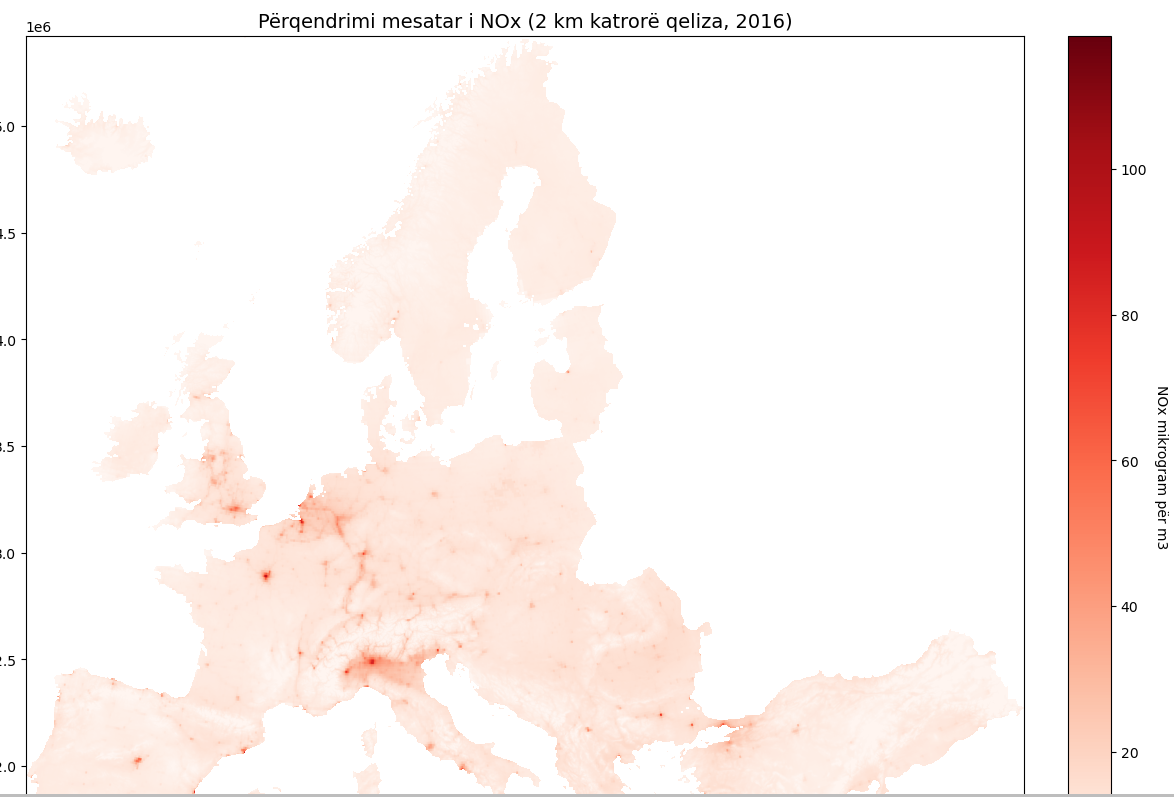
\includegraphics{./Figs/nox.png}
\end{frame}

\begin{frame}{Të dhënat Raster}
\protect\hypertarget{tuxeb-dhuxebnat-raster-8}{}
\begin{itemize}
\item
  Një operacion bazë me raster është të lexosh vlerën në një pikë të
  caktuar.
\item
  Rasteri përfaqëson përqendrimin mesatar vjetor të NOx në 2016, matur
  në mikrogramë për çdo metër kub të ajrit (/m³).
\end{itemize}
\end{frame}

\begin{frame}[fragile]{Të dhënat Raster}
\protect\hypertarget{tuxeb-dhuxebnat-raster-9}{}
\AddToHookNext{env/Highlighting/begin}{\tiny}

\begin{Shaded}
\begin{Highlighting}[]
\CommentTok{\# një pikë në Paris (në projekcionin Lambert)}
\NormalTok{paris\_centroid\_lamb }\OperatorTok{=}\NormalTok{ [}\DecValTok{3758948}\NormalTok{, }\DecValTok{2889291}\NormalTok{]}
\end{Highlighting}
\end{Shaded}
\end{frame}

\begin{frame}[fragile]{Të dhënat Raster}
\protect\hypertarget{tuxeb-dhuxebnat-raster-10}{}
\AddToHookNext{env/Highlighting/begin}{\tiny}

\begin{Shaded}
\begin{Highlighting}[]
\CommentTok{\# Merrni rreshtin/kolonën në raster që korrespondon me vendndodhjen gjeografike paris\_centroid\_lamb}
\NormalTok{loc\_idx }\OperatorTok{=}\NormalTok{ nox\_rast.index(paris\_centroid\_lamb[}\DecValTok{0}\NormalTok{], paris\_centroid\_lamb[}\DecValTok{1}\NormalTok{])}
\BuiltInTok{print}\NormalTok{(}\StringTok{"Vendndodhja e qelizës në raster:"}\NormalTok{, loc\_idx)}
\end{Highlighting}
\end{Shaded}
\end{frame}

\begin{frame}[fragile]{Të dhënat Raster}
\protect\hypertarget{tuxeb-dhuxebnat-raster-11}{}
\AddToHookNext{env/Highlighting/begin}{\tiny}

\begin{Shaded}
\begin{Highlighting}[]
\CommentTok{\# lexoni vlerën}
\NormalTok{nox\_val }\OperatorTok{=}\NormalTok{ nox\_rast.read(}\DecValTok{1}\NormalTok{)[loc\_idx]}
\BuiltInTok{print}\NormalTok{(}\StringTok{"Vlera e NOx në Paris:"}\NormalTok{, nox\_val)}
\end{Highlighting}
\end{Shaded}
\end{frame}

\begin{frame}{Histogrami i Rasterit}
\protect\hypertarget{histogrami-i-rasterit}{}
\begin{itemize}
\item
  Si gjithmonë, është e rëndësishme të vëzhgoni shpërndarjen e vlerave
  me një histogram.
\item
  Vini re se kufiri i rekomanduar NOx për BE është 40.
\item
  Për fat të mirë, shumica e zonave shfaqen nën atë kufi, por është e
  mundur të vëzhgohen disa qeliza me vlera shumë të larta.
\end{itemize}
\end{frame}

\begin{frame}[fragile]{Histogrami i Rasterit}
\protect\hypertarget{histogrami-i-rasterit-1}{}
\AddToHookNext{env/Highlighting/begin}{\tiny}

\begin{Shaded}
\begin{Highlighting}[]
\ImportTok{from}\NormalTok{ rasterio.plot }\ImportTok{import}\NormalTok{ show\_hist}

\CommentTok{\# Shfaq histogramin e vlerave të rasterit}
\NormalTok{show\_hist(nox\_rast, bins}\OperatorTok{=}\DecValTok{20}\NormalTok{, lw}\OperatorTok{=}\FloatTok{0.0}\NormalTok{, stacked}\OperatorTok{=}\VariableTok{False}\NormalTok{, alpha}\OperatorTok{=}\FloatTok{0.3}\NormalTok{, label}\OperatorTok{=}\StringTok{\textquotesingle{}Nr. i qelizave\textquotesingle{}}\NormalTok{,}
\NormalTok{    histtype}\OperatorTok{=}\StringTok{\textquotesingle{}stepfilled\textquotesingle{}}\NormalTok{, title}\OperatorTok{=}\StringTok{"Vlerat e NOx në BE (2016)"}\NormalTok{)}
\end{Highlighting}
\end{Shaded}
\end{frame}

\begin{frame}{Riklasifikimi i Rasterit}
\protect\hypertarget{riklasifikimi-i-rasterit}{}
\begin{itemize}
\tightlist
\item
  Në brendësi, një grup të dhënash raster në Python është një objekt i
  tipit \textbf{numpy.ndarray}, nga paketa \textbf{numpy}.
\end{itemize}
\end{frame}

\begin{frame}{Riklasifikimi i Rasterit}
\protect\hypertarget{riklasifikimi-i-rasterit-1}{}
\begin{itemize}
\tightlist
\item
  Kemi të bëjmë me një \textbf{masiv} shumëdimensional, i cili është një
  mënyrë intuitive për të përfaqësuar grupet e të dhënave raster me
  shumë banda.
\end{itemize}
\end{frame}

\begin{frame}{Riklasifikimi i Rasterit}
\protect\hypertarget{riklasifikimi-i-rasterit-2}{}
\begin{itemize}
\item
  Kjo strukturë e fuqishme e të dhënave përdoret shumë për llogaritje
  shkencore sepse supporton operacione të shpejta në rreshta dhe kolona.
\item
  Për shembull, ne mund të numërojmë dhe tregojmë zona me NOx
  \textgreater{} 40.
\end{itemize}
\end{frame}

\begin{frame}{Riklasifikimi i Rasterit}
\protect\hypertarget{riklasifikimi-i-rasterit-3}{}
\begin{itemize}
\tightlist
\item
  \textbf{Riklasifikimi} i një rasteri është një operacion i zakonshëm
  ku prodhohet një raster i ri bazuar në një klasifikim:
\end{itemize}
\end{frame}

\begin{frame}{Riklasifikimi i Rasterit}
\protect\hypertarget{riklasifikimi-i-rasterit-4}{}
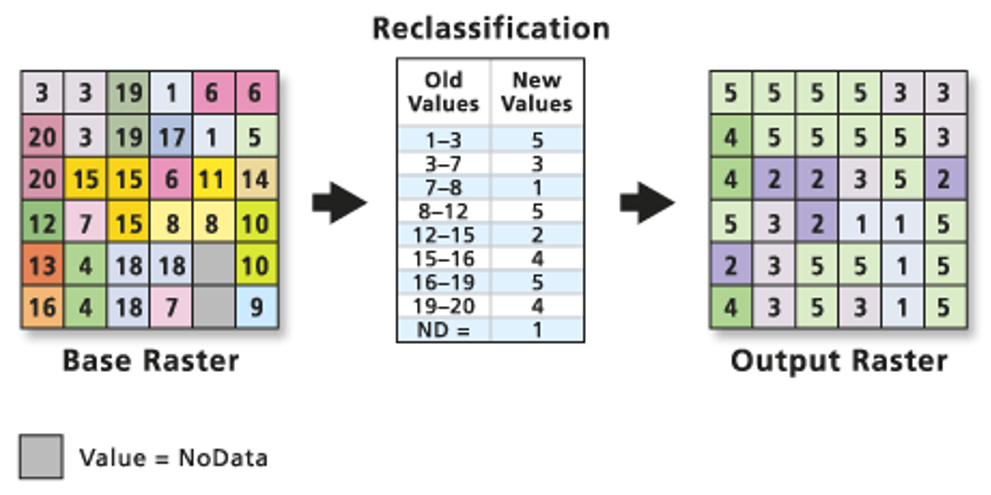
\includegraphics{./Figs/reclassify1.png} \#\# Riklasifikimi i Rasterit

Për NOx, po riklasifikojmë rasterin sipas kategorive:

\begin{itemize}
\item
  {[}0, 20): low (cat = 1)
\item
  {[}20, 40): medium (cat = 2)
\item
  {[}40, 60): high (cat = 3)
\item
  {[}60, ): critical (cat = 4)
\end{itemize}
\end{frame}

\begin{frame}[fragile]{Histogrami i Rasterit}
\protect\hypertarget{histogrami-i-rasterit-2}{}
\AddToHookNext{env/Highlighting/begin}{\tiny}

\begin{Shaded}
\begin{Highlighting}[]
\CommentTok{\# Merr matricën me vlerat e rasterit}
\NormalTok{vals }\OperatorTok{=}\NormalTok{ nox\_rast.read(}\DecValTok{1}\NormalTok{, masked}\OperatorTok{=}\VariableTok{True}\NormalTok{)}
\BuiltInTok{print}\NormalTok{(}\BuiltInTok{type}\NormalTok{(vals))}
\BuiltInTok{print}\NormalTok{(}\StringTok{"Madhësia e matricës:"}\NormalTok{, vals.shape)  }\CommentTok{\# x y}
\end{Highlighting}
\end{Shaded}
\end{frame}

\begin{frame}[fragile]{Histogrami i Rasterit}
\protect\hypertarget{histogrami-i-rasterit-3}{}
\AddToHookNext{env/Highlighting/begin}{\tiny}

\begin{Shaded}
\begin{Highlighting}[]
\CommentTok{\# Zgjidhni vetëm vlerat \textgreater{} 40}
\NormalTok{high\_vals }\OperatorTok{=}\NormalTok{ vals[vals }\OperatorTok{\textgreater{}} \DecValTok{40}\NormalTok{]}
\BuiltInTok{print}\NormalTok{(}\BuiltInTok{len}\NormalTok{(high\_vals), }\StringTok{\textquotesingle{}qeliza kanë vlera të larta të NOx (\textgreater{}40 mikrogram/m³).\textquotesingle{}}\NormalTok{)}
\BuiltInTok{print}\NormalTok{(}\StringTok{\textquotesingle{}}\SpecialCharTok{\% e}\StringTok{ totalit të qelizave:\textquotesingle{}}\NormalTok{, (}\BuiltInTok{len}\NormalTok{(high\_vals) }\OperatorTok{/}\NormalTok{ (vals.shape[}\DecValTok{0}\NormalTok{] }\OperatorTok{*}\NormalTok{ vals.shape[}\DecValTok{1}\NormalTok{])) }\OperatorTok{*} \DecValTok{100}\NormalTok{)}
\end{Highlighting}
\end{Shaded}
\end{frame}

\begin{frame}[fragile]{Histogrami i Rasterit}
\protect\hypertarget{histogrami-i-rasterit-4}{}
\AddToHookNext{env/Highlighting/begin}{\tiny}

\begin{Shaded}
\begin{Highlighting}[]
\CommentTok{\# Riklasifikimi:}
\CommentTok{\# Kopjoni matricën për të ruajtur të dhënat origjinale}
\NormalTok{recl\_vals }\OperatorTok{=}\NormalTok{ vals.copy()}
\end{Highlighting}
\end{Shaded}
\end{frame}

\begin{frame}[fragile]{Histogrami i Rasterit}
\protect\hypertarget{histogrami-i-rasterit-5}{}
\AddToHookNext{env/Highlighting/begin}{\tiny}

\begin{Shaded}
\begin{Highlighting}[]
\CommentTok{\# Zbato klasifikimin e ri (4 = vlera shumë të larta)}
\CommentTok{\# Vini re se renditja e këtyre veprimeve është e rëndësishme për të realizuar një}
\CommentTok{\# riklasifikim të saktë.}
\NormalTok{recl\_vals[vals }\OperatorTok{\textgreater{}} \DecValTok{0}\NormalTok{] }\OperatorTok{=} \DecValTok{4}
\CommentTok{\# nëse vals \textless{} 60 vendos vlerën në 3}
\NormalTok{recl\_vals[vals }\OperatorTok{\textless{}} \DecValTok{60}\NormalTok{] }\OperatorTok{=} \DecValTok{3}
\CommentTok{\# nëse vals \textless{} 40 vendos vlerën në 2}
\NormalTok{recl\_vals[vals }\OperatorTok{\textless{}} \DecValTok{40}\NormalTok{] }\OperatorTok{=} \DecValTok{2}
\CommentTok{\# nëse vals \textless{} 20 vendos vlerën në 1}
\NormalTok{recl\_vals[vals }\OperatorTok{\textless{}} \DecValTok{20}\NormalTok{] }\OperatorTok{=} \DecValTok{1}

\CommentTok{\# Shfaq rezultatin}
\NormalTok{plot\_raster(nox\_rast, recl\_vals, }\StringTok{\textquotesingle{}Përqendrimi mesatar i NOx (2 km² qeliza, 2016)\textquotesingle{}}\NormalTok{, }
    \StringTok{\textquotesingle{}Kategoritë e përqendrimit të NOx (4=max)\textquotesingle{}}\NormalTok{, cmap}\OperatorTok{=}\StringTok{\textquotesingle{}Blues\textquotesingle{}}\NormalTok{, width}\OperatorTok{=}\DecValTok{14}\NormalTok{, height}\OperatorTok{=}\DecValTok{14}\NormalTok{)}
\end{Highlighting}
\end{Shaded}
\end{frame}

\begin{frame}{Libraria xarray}
\protect\hypertarget{libraria-xarray}{}
\begin{itemize}
\item
  \textbf{xarray} është një bibliotekë në Python e specializuar për
  analizën dhe manipulimin e të dhënave shumë-dimensionale (në stilin e
  Pandas), e përshtatshme për dataset-e të mëdha, si p.sh., të dhënat
  klimatike apo ato të analizës së rastereve.
\item
  Ofron support të plotë për struktura të avancuara të të dhënave dhe
  sisteme të ndryshme koordinative, duke lejuar qasje të lehtë dhe
  efikase në analiza dhe vizualizim të avancuar.
\end{itemize}
\end{frame}

\begin{frame}{Libraria xarray}
\protect\hypertarget{libraria-xarray-1}{}
\begin{itemize}
\item
  \textbf{rioxarray} është një bibliotekë Python që zgjeron
  funksionalitetin e \textbf{xarray} për të suportuar të dhëna
  gjeohapësinore, duke lejuar leximin, manipulimin dhe analizimin e të
  dhënave raster me lehtësi.
\item
  Ajo integron kapacitetet e \textbf{rasterio} në kornizën fleksibël të
  \textbf{xarray}, duke e bërë punën me të dhënat gjeohapësinore më të
  fuqishme dhe efikase.
\end{itemize}
\end{frame}

\begin{frame}[fragile]{Instalim}
\protect\hypertarget{instalim}{}
\begin{Shaded}
\begin{Highlighting}[]
\NormalTok{conda install rioxarray}
\end{Highlighting}
\end{Shaded}
\end{frame}

\begin{frame}{Shembull}
\protect\hypertarget{shembull}{}
\begin{itemize}
\item
  Bandat \textbf{Landsat 8} ruhen si skedarë të veçantë GeoTIFF në
  paketën origjinale.
\item
  Çdo brez përmban informacion të reflektimit të sipërfaqes nga diapazon
  të ndryshëm të spektrit elektromagnetik.
\end{itemize}
\end{frame}

\begin{frame}[fragile]{Shkarkimi i të Dhënave}
\protect\hypertarget{shkarkimi-i-tuxeb-dhuxebnave}{}
\AddToHookNext{env/Highlighting/begin}{\tiny}

\begin{Shaded}
\begin{Highlighting}[]
\ImportTok{import}\NormalTok{ rioxarray}
\ImportTok{import}\NormalTok{ matplotlib.pyplot }\ImportTok{as}\NormalTok{ plt}

\CommentTok{\# Hapni skedarin raster duke përdorur rioxarray}
\NormalTok{url }\OperatorTok{=} \StringTok{"https://a3s.fi/swift/v1/AUTH\_0914d8aff9684df589041a759b549fc2/PythonGIS/elevation/kilimanjaro/ASTGTMV003\_S03E036\_dem.tif"}
\NormalTok{data }\OperatorTok{=}\NormalTok{ rioxarray.open\_rasterio(url, masked}\OperatorTok{=}\VariableTok{True}\NormalTok{)}
\end{Highlighting}
\end{Shaded}
\end{frame}

\begin{frame}[fragile]{Vizualizoni}
\protect\hypertarget{vizualizoni}{}
\AddToHookNext{env/Highlighting/begin}{\tiny}

\begin{Shaded}
\begin{Highlighting}[]
\NormalTok{data.plot()}
\NormalTok{plt.title(}\StringTok{"Elevacioni i Kilimanjaros"}\NormalTok{)}
\NormalTok{plt.show()}
\end{Highlighting}
\end{Shaded}
\end{frame}

\begin{frame}{Vizualizoni}
\protect\hypertarget{vizualizoni-1}{}
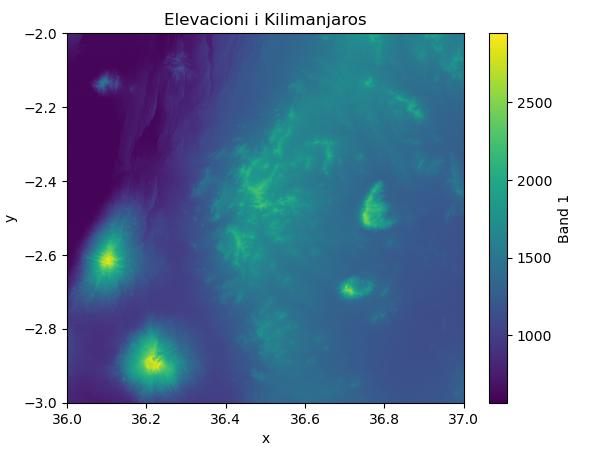
\includegraphics{./Figs/kilima.png}
\end{frame}

\begin{frame}[fragile]{Hapja e File-it Raster}
\protect\hypertarget{hapja-e-file-it-raster}{}
\AddToHookNext{env/Highlighting/begin}{\tiny}

\begin{Shaded}
\begin{Highlighting}[]
\ImportTok{import}\NormalTok{ rasterio}
\ImportTok{import}\NormalTok{ os}
\ImportTok{import}\NormalTok{ numpy }\ImportTok{as}\NormalTok{ np}

\CommentTok{\# Direktoria e të dhënave}
\NormalTok{data\_dir }\OperatorTok{=} \StringTok{"data/gis3"}
\NormalTok{fp }\OperatorTok{=}\NormalTok{ os.path.join(data\_dir, }\StringTok{"Helsinki\_masked\_p188r018\_7t20020529\_z34\_\_LV{-}FIN.tif"}\NormalTok{)}

\CommentTok{\# Hapni file{-}in}
\NormalTok{raster }\OperatorTok{=}\NormalTok{ rasterio.}\BuiltInTok{open}\NormalTok{(fp)}
\end{Highlighting}
\end{Shaded}
\end{frame}

\begin{frame}[fragile]{Kontrolloni llojin e variablit `raster'}
\protect\hypertarget{kontrolloni-llojin-e-variablit-raster}{}
\AddToHookNext{env/Highlighting/begin}{\tiny}

\begin{Shaded}
\begin{Highlighting}[]
\BuiltInTok{type}\NormalTok{(raster)}
\end{Highlighting}
\end{Shaded}
\end{frame}

\begin{frame}[fragile]{Leximi i Karakteristikave të File-it Raster}
\protect\hypertarget{leximi-i-karakteristikave-tuxeb-file-it-raster}{}
\AddToHookNext{env/Highlighting/begin}{\tiny}

\begin{Shaded}
\begin{Highlighting}[]
\CommentTok{\# Projeksioni}
\NormalTok{raster.crs}
\end{Highlighting}
\end{Shaded}
\end{frame}

\begin{frame}[fragile]{Transformimi affine (si rregullohet, rrotullohet,
apo zhvendoset rasteri)}
\protect\hypertarget{transformimi-affine-si-rregullohet-rrotullohet-apo-zhvendoset-rasteri}{}
\AddToHookNext{env/Highlighting/begin}{\tiny}

\begin{Shaded}
\begin{Highlighting}[]
\NormalTok{raster.transform}
\end{Highlighting}
\end{Shaded}
\end{frame}

\begin{frame}[fragile]{Dimensionet}
\protect\hypertarget{dimensionet}{}
\AddToHookNext{env/Highlighting/begin}{\tiny}

\begin{Shaded}
\begin{Highlighting}[]
\BuiltInTok{print}\NormalTok{(raster.width)}
\BuiltInTok{print}\NormalTok{(raster.height)}
\end{Highlighting}
\end{Shaded}
\end{frame}

\begin{frame}[fragile]{Numri i bandave}
\protect\hypertarget{numri-i-bandave}{}
\AddToHookNext{env/Highlighting/begin}{\tiny}

\begin{Shaded}
\begin{Highlighting}[]
\CommentTok{\# Numri i bandave}
\NormalTok{raster.count}
\end{Highlighting}
\end{Shaded}
\end{frame}

\begin{frame}[fragile]{Kufijtë e file-it}
\protect\hypertarget{kufijtuxeb-e-file-it}{}
\AddToHookNext{env/Highlighting/begin}{\tiny}

\begin{Shaded}
\begin{Highlighting}[]
\NormalTok{raster.bounds}
\end{Highlighting}
\end{Shaded}
\end{frame}

\begin{frame}[fragile]{Driver-i (formati i të dhënave)}
\protect\hypertarget{driver-i-formati-i-tuxeb-dhuxebnave}{}
\AddToHookNext{env/Highlighting/begin}{\tiny}

\begin{Shaded}
\begin{Highlighting}[]
\NormalTok{raster.driver}
\end{Highlighting}
\end{Shaded}
\end{frame}

\begin{frame}[fragile]{Vlerat pa të dhëna për të gjitha kanalet}
\protect\hypertarget{vlerat-pa-tuxeb-dhuxebna-puxebr-tuxeb-gjitha-kanalet}{}
\AddToHookNext{env/Highlighting/begin}{\tiny}

\begin{Shaded}
\begin{Highlighting}[]
\NormalTok{raster.nodatavals}
\end{Highlighting}
\end{Shaded}
\end{frame}

\begin{frame}[fragile]{Të gjitha Meta të Dhënat për dataset-in e
rasterit}
\protect\hypertarget{tuxeb-gjitha-meta-tuxeb-dhuxebnat-puxebr-dataset-in-e-rasterit}{}
\AddToHookNext{env/Highlighting/begin}{\tiny}

\begin{Shaded}
\begin{Highlighting}[]
\NormalTok{raster.meta}
\end{Highlighting}
\end{Shaded}
\end{frame}

\begin{frame}[fragile]{Marrja e Brezeve të Rasterit}
\protect\hypertarget{marrja-e-brezeve-tuxeb-rasterit}{}
\AddToHookNext{env/Highlighting/begin}{\tiny}

\begin{Shaded}
\begin{Highlighting}[]
\CommentTok{\# Lexoni brezrin e rasterit si variabël të veçantë}
\NormalTok{band1 }\OperatorTok{=}\NormalTok{ raster.read(}\DecValTok{1}\NormalTok{)}
\end{Highlighting}
\end{Shaded}
\end{frame}

\begin{frame}[fragile]{Kontrolloni llojin e variablit `band'}
\protect\hypertarget{kontrolloni-llojin-e-variablit-band}{}
\AddToHookNext{env/Highlighting/begin}{\tiny}

\begin{Shaded}
\begin{Highlighting}[]
\BuiltInTok{print}\NormalTok{(}\BuiltInTok{type}\NormalTok{(band1))}

\CommentTok{\# Lloji i të dhënave të vlerave}
\BuiltInTok{print}\NormalTok{(band1.dtype)}
\end{Highlighting}
\end{Shaded}
\end{frame}

\begin{frame}[fragile]{Statistikat e Brezit}
\protect\hypertarget{statistikat-e-brezit}{}
\AddToHookNext{env/Highlighting/begin}{\tiny}

\begin{Shaded}
\begin{Highlighting}[]
\CommentTok{\# Lexoni të gjithë brezin}
\NormalTok{array }\OperatorTok{=}\NormalTok{ raster.read()}
\end{Highlighting}
\end{Shaded}
\end{frame}

\begin{frame}[fragile]{Llogarisni statistikat për çdo brez}
\protect\hypertarget{llogarisni-statistikat-puxebr-uxe7do-brez}{}
\AddToHookNext{env/Highlighting/begin}{\tiny}

\begin{Shaded}
\begin{Highlighting}[]
\NormalTok{stats }\OperatorTok{=}\NormalTok{ []}
\ControlFlowTok{for}\NormalTok{ band }\KeywordTok{in}\NormalTok{ array:}
\NormalTok{    stats.append(}
\NormalTok{        \{}
            \StringTok{"min"}\NormalTok{: band.}\BuiltInTok{min}\NormalTok{(),}
            \StringTok{"mean"}\NormalTok{: band.mean(),}
            \StringTok{"median"}\NormalTok{: np.median(band),}
            \StringTok{"max"}\NormalTok{: band.}\BuiltInTok{max}\NormalTok{(),}
\NormalTok{        \}}
\NormalTok{    )}
\end{Highlighting}
\end{Shaded}
\end{frame}

\begin{frame}[fragile]{Shfaqni statistikat për çdo kanal}
\protect\hypertarget{shfaqni-statistikat-puxebr-uxe7do-kanal}{}
\AddToHookNext{env/Highlighting/begin}{\tiny}

\begin{Shaded}
\begin{Highlighting}[]
\NormalTok{stats}
\end{Highlighting}
\end{Shaded}
\end{frame}

\begin{frame}{Krijimi i një Mozaiku Raster}
\protect\hypertarget{krijimi-i-njuxeb-mozaiku-raster}{}
\begin{itemize}
\item
  Shumë shpesh ju duhet të bashkoni së bashku skedarë të shumtë raster
  dhe të krijoni një mozaik raster \textbf{raster mosaic}.
\item
  Kjo mund të bëhet lehtësisht me funksionin \textbf{merge\_datasets()}
  -në \textbf{rioxarray}.
\item
  Këtu, ne do të krijojmë një mozaik bazuar në skedarët \textbf{DEM}
  (gjithsej 4 skedarë) që mbulojnë rajonin e Kilimanjaros në Tanzani.
\end{itemize}
\end{frame}

\begin{frame}[fragile]{Krijimi i një Mozaiku Raster}
\protect\hypertarget{krijimi-i-njuxeb-mozaiku-raster-1}{}
Së pari do të lexojmë të dhënat e lartësisë nga një kovë S3 për rajonin
e Kilimanxharos në Afrikë.

\AddToHookNext{env/Highlighting/begin}{\tiny}

\begin{Shaded}
\begin{Highlighting}[]
\ImportTok{import}\NormalTok{ xarray }\ImportTok{as}\NormalTok{ xr}
\ImportTok{import}\NormalTok{ os}
\ImportTok{import}\NormalTok{ rioxarray }\ImportTok{as}\NormalTok{ rxr}
\ImportTok{from}\NormalTok{ rioxarray.merge }\ImportTok{import}\NormalTok{ merge\_datasets}

\CommentTok{\# S3 bucket që përmban të dhënat}
\NormalTok{bucket }\OperatorTok{=} \StringTok{"https://a3s.fi/swift/v1/AUTH\_0914d8aff9684df589041a759b549fc2/PythonGIS"}

\CommentTok{\# Gjeneroni URL{-}të për skedarët e lartësisë}
\NormalTok{urls }\OperatorTok{=}\NormalTok{ [}
\NormalTok{    os.path.join(bucket, }\StringTok{"elevation/kilimanjaro/ASTGTMV003\_S03E036\_dem.tif"}\NormalTok{),}
\NormalTok{    os.path.join(bucket, }\StringTok{"elevation/kilimanjaro/ASTGTMV003\_S03E037\_dem.tif"}\NormalTok{),}
\NormalTok{    os.path.join(bucket, }\StringTok{"elevation/kilimanjaro/ASTGTMV003\_S04E036\_dem.tif"}\NormalTok{),}
\NormalTok{    os.path.join(bucket, }\StringTok{"elevation/kilimanjaro/ASTGTMV003\_S04E037\_dem.tif"}\NormalTok{),}
\NormalTok{]}
\end{Highlighting}
\end{Shaded}
\end{frame}

\begin{frame}[fragile]{Krijimi i një Mozaiku Raster}
\protect\hypertarget{krijimi-i-njuxeb-mozaiku-raster-2}{}
\AddToHookNext{env/Highlighting/begin}{\tiny}

\begin{Shaded}
\begin{Highlighting}[]
\CommentTok{\# Lexoni skedarët}
\NormalTok{datasets }\OperatorTok{=}\NormalTok{ [}
\NormalTok{    xr.open\_dataset(url, engine}\OperatorTok{=}\StringTok{"rasterio"}\NormalTok{).squeeze(}\StringTok{"band"}\NormalTok{, drop}\OperatorTok{=}\VariableTok{True}\NormalTok{) }\ControlFlowTok{for}\NormalTok{ url }\KeywordTok{in}\NormalTok{ urls}
\NormalTok{]}
\end{Highlighting}
\end{Shaded}
\end{frame}

\begin{frame}[fragile]{Vizualizimi i Pllakave (Tiles)}
\protect\hypertarget{vizualizimi-i-pllakave-tiles}{}
Shohim fillimisht si duken të dhënat:

\begin{Shaded}
\begin{Highlighting}[]
\NormalTok{datasets[}\DecValTok{0}\NormalTok{]}
\end{Highlighting}
\end{Shaded}
\end{frame}

\begin{frame}{Vizualizimi i Pllakave (Tiles)}
\protect\hypertarget{vizualizimi-i-pllakave-tiles-1}{}
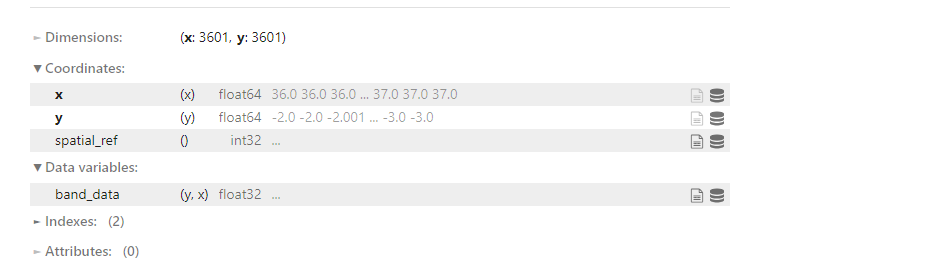
\includegraphics{./Figs/tiless.png}
\end{frame}

\begin{frame}[fragile]{Vizualizimi i Pllakave (Tiles)}
\protect\hypertarget{vizualizimi-i-pllakave-tiles-2}{}
\AddToHookNext{env/Highlighting/begin}{\tiny}

\begin{Shaded}
\begin{Highlighting}[]
\ImportTok{import}\NormalTok{ matplotlib.pyplot }\ImportTok{as}\NormalTok{ plt}

\CommentTok{\# Vizualizoni dërrasat për të parë se si duken veç e veç}
\NormalTok{fig, axes }\OperatorTok{=}\NormalTok{ plt.subplots(}\DecValTok{2}\NormalTok{, }\DecValTok{2}\NormalTok{, figsize}\OperatorTok{=}\NormalTok{(}\DecValTok{16}\NormalTok{, }\DecValTok{16}\NormalTok{))}
\NormalTok{datasets[}\DecValTok{0}\NormalTok{][}\StringTok{"band\_data"}\NormalTok{].plot(ax}\OperatorTok{=}\NormalTok{axes[}\DecValTok{0}\NormalTok{][}\DecValTok{0}\NormalTok{], vmax}\OperatorTok{=}\DecValTok{5900}\NormalTok{, add\_colorbar}\OperatorTok{=}\VariableTok{False}\NormalTok{)}
\NormalTok{datasets[}\DecValTok{1}\NormalTok{][}\StringTok{"band\_data"}\NormalTok{].plot(ax}\OperatorTok{=}\NormalTok{axes[}\DecValTok{0}\NormalTok{][}\DecValTok{1}\NormalTok{], vmax}\OperatorTok{=}\DecValTok{5900}\NormalTok{, add\_colorbar}\OperatorTok{=}\VariableTok{False}\NormalTok{)}
\NormalTok{datasets[}\DecValTok{2}\NormalTok{][}\StringTok{"band\_data"}\NormalTok{].plot(ax}\OperatorTok{=}\NormalTok{axes[}\DecValTok{1}\NormalTok{][}\DecValTok{0}\NormalTok{], vmax}\OperatorTok{=}\DecValTok{5900}\NormalTok{, add\_colorbar}\OperatorTok{=}\VariableTok{False}\NormalTok{)}
\NormalTok{datasets[}\DecValTok{3}\NormalTok{][}\StringTok{"band\_data"}\NormalTok{].plot(ax}\OperatorTok{=}\NormalTok{axes[}\DecValTok{1}\NormalTok{][}\DecValTok{1}\NormalTok{], vmax}\OperatorTok{=}\DecValTok{5900}\NormalTok{, add\_colorbar}\OperatorTok{=}\VariableTok{False}\NormalTok{)}
\end{Highlighting}
\end{Shaded}
\end{frame}

\begin{frame}{Vizualizimi i Pllakave (Tiles)}
\protect\hypertarget{vizualizimi-i-pllakave-tiles-3}{}
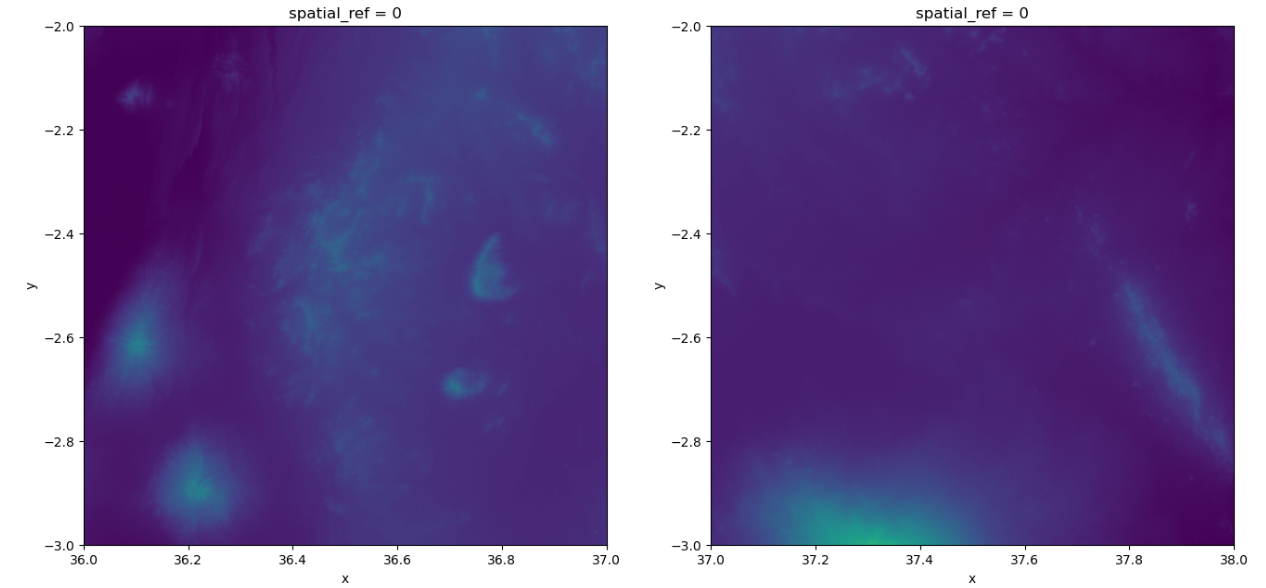
\includegraphics{./Figs/tiles2.png}
\end{frame}

\begin{frame}{Krijimi i Mozaikut Raster}
\protect\hypertarget{krijimi-i-mozaikut-raster}{}
\begin{itemize}
\item
  Siç mund ta shohim ne kemi skedarë të shumtë raster të veçantë që
  ndodhen pranë njëri-tjetrit.
\item
  Prandaj, ne duam t'i bashkojmë ato në një skedar të vetëm raster që
  mund të bëhet duke krijuar një mozaik raster.
\item
  Mund të krijojmë një mozaik raster duke bashkuar këto grupe të dhënash
  me funksionin \textbf{merge\_datasets()}:
\end{itemize}
\end{frame}

\begin{frame}[fragile]{Krijimi i Mozaikut Raster}
\protect\hypertarget{krijimi-i-mozaikut-raster-1}{}
\AddToHookNext{env/Highlighting/begin}{\tiny}

\begin{Shaded}
\begin{Highlighting}[]
\CommentTok{\# Krijoni një mozaik nga dërrasat}
\NormalTok{mosaic }\OperatorTok{=}\NormalTok{ merge\_datasets(datasets)}

\CommentTok{\# Shtoni një emër më intuitiv për variablin e të dhënave}
\NormalTok{mosaic }\OperatorTok{=}\NormalTok{ mosaic.rename(\{}\StringTok{"band\_data"}\NormalTok{: }\StringTok{"elevation"}\NormalTok{\})}
\end{Highlighting}
\end{Shaded}
\end{frame}

\begin{frame}[fragile]{Vizualizoni mozaikun}
\protect\hypertarget{vizualizoni-mozaikun}{}
\AddToHookNext{env/Highlighting/begin}{\tiny}

\begin{Shaded}
\begin{Highlighting}[]
\NormalTok{mosaic[}\StringTok{"elevation"}\NormalTok{].plot(figsize}\OperatorTok{=}\NormalTok{(}\DecValTok{12}\NormalTok{, }\DecValTok{12}\NormalTok{))}
\end{Highlighting}
\end{Shaded}
\end{frame}

\begin{frame}{Vizualizoni mozaikun}
\protect\hypertarget{vizualizoni-mozaikun-1}{}
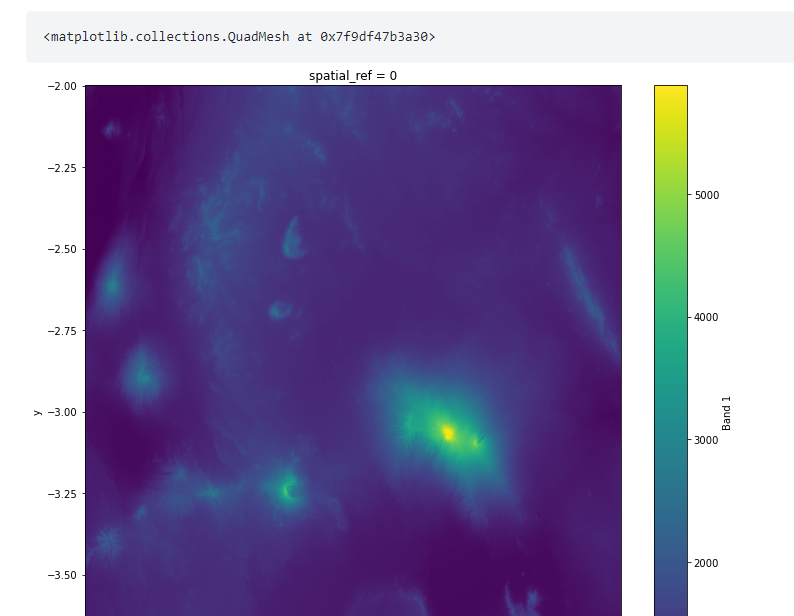
\includegraphics{./Figs/mosaic.png}
\end{frame}

\begin{frame}[fragile]{Prerja e Rasterit}
\protect\hypertarget{prerja-e-rasterit}{}
\AddToHookNext{env/Highlighting/begin}{\tiny}

\begin{Shaded}
\begin{Highlighting}[]
\ImportTok{import}\NormalTok{ geopandas }\ImportTok{as}\NormalTok{ gpd}
\ImportTok{from}\NormalTok{ shapely.geometry }\ImportTok{import}\NormalTok{ box}

\CommentTok{\# Koordinatat e kutisë kufizuese}
\NormalTok{minx }\OperatorTok{=} \FloatTok{37.1}
\NormalTok{miny }\OperatorTok{=} \OperatorTok{{-}}\FloatTok{3.3}
\NormalTok{maxx }\OperatorTok{=} \FloatTok{37.6}
\NormalTok{maxy }\OperatorTok{=} \OperatorTok{{-}}\FloatTok{2.85}
\end{Highlighting}
\end{Shaded}
\end{frame}

\begin{frame}[fragile]{Prerja e Rasterit}
\protect\hypertarget{prerja-e-rasterit-1}{}
\AddToHookNext{env/Highlighting/begin}{\tiny}

\begin{Shaded}
\begin{Highlighting}[]
\CommentTok{\# Krijoni një GeoDataFrame që do të përdoret për të prerë rasterin}
\NormalTok{geom }\OperatorTok{=}\NormalTok{ box(minx, miny, maxx, maxy)}
\NormalTok{clipping\_gdf }\OperatorTok{=}\NormalTok{ gpd.GeoDataFrame(\{}\StringTok{"geometry"}\NormalTok{: [geom]\}, index}\OperatorTok{=}\NormalTok{[}\DecValTok{0}\NormalTok{], crs}\OperatorTok{=}\StringTok{"epsg:4326"}\NormalTok{)}
\end{Highlighting}
\end{Shaded}
\end{frame}

\begin{frame}[fragile]{Prerja e Rasterit}
\protect\hypertarget{prerja-e-rasterit-2}{}
\AddToHookNext{env/Highlighting/begin}{\tiny}

\begin{Shaded}
\begin{Highlighting}[]
\CommentTok{\# Eksploroni shtrirjen në hartë}
\NormalTok{clipping\_gdf.explore()}
\end{Highlighting}
\end{Shaded}
\end{frame}

\begin{frame}{Prerja e Rasterit}
\protect\hypertarget{prerja-e-rasterit-3}{}
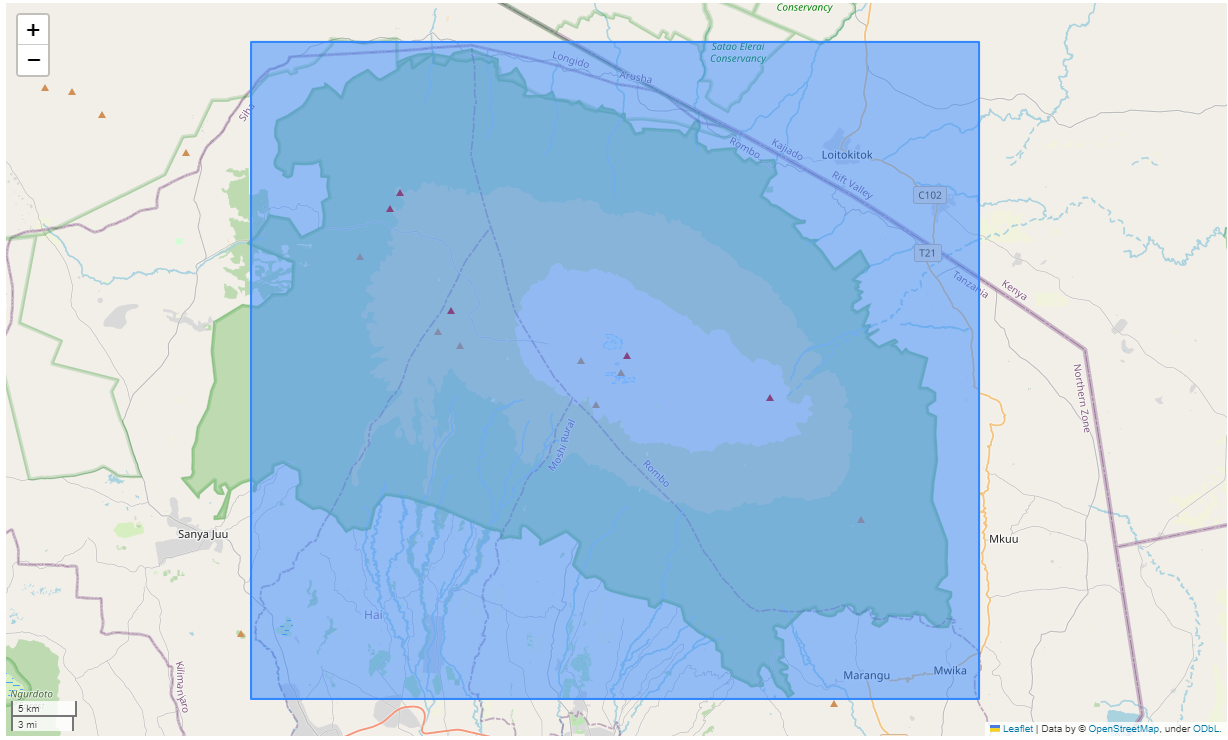
\includegraphics{./Figs/mosaic2.png}
\end{frame}

\begin{frame}[fragile]{Prerja e Mozaikut me GeoDataFrame}
\protect\hypertarget{prerja-e-mozaikut-me-geodataframe}{}
\AddToHookNext{env/Highlighting/begin}{\tiny}

\begin{Shaded}
\begin{Highlighting}[]
\CommentTok{\# Priteni mozaikun me GeoDataFrame dhe specifikoni CRS}
\NormalTok{kilimanjaro }\OperatorTok{=}\NormalTok{ mosaic.rio.clip(clipping\_gdf.geometry, crs}\OperatorTok{=}\NormalTok{mosaic.elevation.rio.crs)}
\NormalTok{kilimanjaro[}\StringTok{"elevation"}\NormalTok{].plot()}
\end{Highlighting}
\end{Shaded}
\end{frame}

\begin{frame}{Prerja e Mozaikut me GeoDataFrame}
\protect\hypertarget{prerja-e-mozaikut-me-geodataframe-1}{}
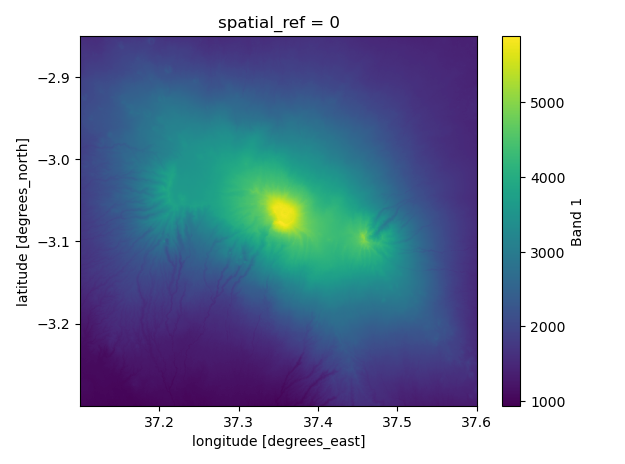
\includegraphics{./Figs/mosaic3.png}
\end{frame}

\begin{frame}[fragile]{Ruajtja e Rasterit në një GeoTIFF}
\protect\hypertarget{ruajtja-e-rasterit-nuxeb-njuxeb-geotiff}{}
\AddToHookNext{env/Highlighting/begin}{\tiny}

\begin{Shaded}
\begin{Highlighting}[]
\CommentTok{\# Ruani file{-}in në GeoTIFF}
\NormalTok{kilimanjaro.rio.to\_raster(}\StringTok{"data/kilimanjaro.tif"}\NormalTok{, compress}\OperatorTok{=}\StringTok{"LZMA"}\NormalTok{, tiled}\OperatorTok{=}\VariableTok{True}\NormalTok{)}
\end{Highlighting}
\end{Shaded}
\end{frame}

\hypertarget{analiza-e-modeleve-dixhitale-tuxeb-lartuxebsisuxeb-dem}{%
\section{Analiza e Modeleve Dixhitale të Lartësisë
(DEM)}\label{analiza-e-modeleve-dixhitale-tuxeb-lartuxebsisuxeb-dem}}

\begin{frame}{Shkarkimi i Skedarit DEM}
\protect\hypertarget{shkarkimi-i-skedarit-dem}{}
\begin{itemize}
\item
  \textbf{DEM} janë një lloj i zakonshëm i rasterit që përfaqëson
  lartësinë.
\item
  Ky grup të dhënash përfaqëson lartësinë e Himalajeve në një rezolucion
  prej 1 km
\end{itemize}
\end{frame}

\begin{frame}[fragile]{Shkarkimi i Skedarit DEM}
\protect\hypertarget{shkarkimi-i-skedarit-dem-1}{}
\AddToHookNext{env/Highlighting/begin}{\tiny}

\begin{Shaded}
\begin{Highlighting}[]
\ImportTok{import}\NormalTok{ urllib.request}

\CommentTok{\# Shkarkoni file{-}in nga \textquotesingle{}url\textquotesingle{} dhe ruajeni lokalisht nën \textquotesingle{}file\_name\textquotesingle{}}
\NormalTok{url }\OperatorTok{=} \StringTok{\textquotesingle{}https://github.com/andrea{-}ballatore/open{-}geo{-}data{-}education/blob/main/datasets/digital\_elevation\_models/dem\_srtm\_1km\_himalayas\_2009.tif?raw=true\textquotesingle{}}
\NormalTok{rast\_file\_name }\OperatorTok{=} \StringTok{\textquotesingle{}data/dem\_srtm\_1km\_himalayas\_2009.tif\textquotesingle{}}
\NormalTok{urllib.request.urlretrieve(url, rast\_file\_name)}
\end{Highlighting}
\end{Shaded}
\end{frame}

\begin{frame}[fragile]{Hapja dhe Vizualizimi i DEM}
\protect\hypertarget{hapja-dhe-vizualizimi-i-dem}{}
\AddToHookNext{env/Highlighting/begin}{\tiny}

\begin{Shaded}
\begin{Highlighting}[]
\ImportTok{import}\NormalTok{ rasterio}

\CommentTok{\# Hapni file{-}in DEM duke përdorur rasterio}
\NormalTok{him\_rast }\OperatorTok{=}\NormalTok{ rasterio.}\BuiltInTok{open}\NormalTok{(}\StringTok{\textquotesingle{}data/dem\_srtm\_1km\_himalayas\_2009.tif\textquotesingle{}}\NormalTok{)}
\end{Highlighting}
\end{Shaded}
\end{frame}

\begin{frame}[fragile]{Hapja dhe Vizualizimi i DEM}
\protect\hypertarget{hapja-dhe-vizualizimi-i-dem-1}{}
\AddToHookNext{env/Highlighting/begin}{\tiny}

\begin{Shaded}
\begin{Highlighting}[]
\CommentTok{\# Shfaqni informacionin e file{-}it}
\BuiltInTok{print}\NormalTok{(him\_rast.meta)}
\BuiltInTok{print}\NormalTok{(him\_rast.bounds)}
\end{Highlighting}
\end{Shaded}
\end{frame}

\begin{frame}[fragile]{Shfaqja e Vlerave të DEM}
\protect\hypertarget{shfaqja-e-vlerave-tuxeb-dem}{}
\AddToHookNext{env/Highlighting/begin}{\tiny}

\begin{Shaded}
\begin{Highlighting}[]
\CommentTok{\# Vini re se duhet të lexojmë një brez (sepse rasterio nuk e ngarkon atë)}
\NormalTok{vals }\OperatorTok{=}\NormalTok{ him\_rast.read(}\DecValTok{1}\NormalTok{, masked}\OperatorTok{=}\VariableTok{True}\NormalTok{)}
\end{Highlighting}
\end{Shaded}
\end{frame}

\begin{frame}[fragile]{Shfaqni statistika bazë}
\protect\hypertarget{shfaqni-statistika-bazuxeb}{}
\AddToHookNext{env/Highlighting/begin}{\tiny}

\begin{Shaded}
\begin{Highlighting}[]
\BuiltInTok{print}\NormalTok{(}\StringTok{"Vlera minimale (m):"}\NormalTok{, vals.}\BuiltInTok{min}\NormalTok{())}
\CommentTok{\# vini re se për median përdorim np.median}
\BuiltInTok{print}\NormalTok{(}\StringTok{"Vlera mesatare (m):"}\NormalTok{, np.median(vals))}
\BuiltInTok{print}\NormalTok{(}\StringTok{"Vlera maksimale (m):"}\NormalTok{, vals.}\BuiltInTok{max}\NormalTok{())}
\end{Highlighting}
\end{Shaded}
\end{frame}

\begin{frame}[fragile]{Ndërtojmë}
\protect\hypertarget{nduxebrtojmuxeb}{}
\AddToHookNext{env/Highlighting/begin}{\tiny}

\begin{Shaded}
\begin{Highlighting}[]
\NormalTok{plot\_raster(him\_rast, vals, }\StringTok{\textquotesingle{}Himalaya DEM (rezolucion 1km, 2009)\textquotesingle{}}\NormalTok{, }\StringTok{\textquotesingle{}Elevation (m)\textquotesingle{}}\NormalTok{)}
\end{Highlighting}
\end{Shaded}
\end{frame}

\begin{frame}{Ndërtojmë}
\protect\hypertarget{nduxebrtojmuxeb-1}{}
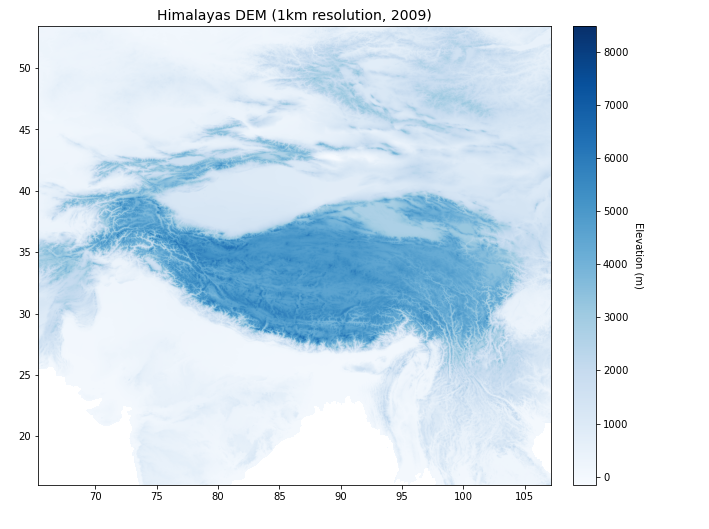
\includegraphics{./Figs/himal3.png}
\end{frame}

\hypertarget{operacione-dem-me-gdal}{%
\section{Operacione DEM me GDAL}\label{operacione-dem-me-gdal}}

\begin{frame}[fragile]{Operacione DEM me GDAL}
\protect\hypertarget{operacione-dem-me-gdal-1}{}
\begin{itemize}
\item
  GDAL mund të përdoret për të kryer operacione të thjeshta në DEM pa i
  ngarkuar ato tërësisht në memorje.
\item
  \texttt{gdal.DEMProcessing(...)} mbështet operacione të zakonshme si
  aspekti, pjerrësia dhe hijezimi i kodrës.
\end{itemize}
\end{frame}

\begin{frame}[fragile]{Përgatitja e Mjedisit}
\protect\hypertarget{puxebrgatitja-e-mjedisit}{}
\AddToHookNext{env/Highlighting/begin}{\tiny}

\begin{Shaded}
\begin{Highlighting}[]
\CommentTok{\# Importoni paketën GDAL dhe rasterio}
\ImportTok{from}\NormalTok{ osgeo }\ImportTok{import}\NormalTok{ gdal}
\ImportTok{import}\NormalTok{ rasterio}
\ImportTok{import}\NormalTok{ os}

\CommentTok{\# Sigurohuni që drejtoria e daljes ekziston}
\NormalTok{os.makedirs(}\StringTok{\textquotesingle{}tmp\textquotesingle{}}\NormalTok{, exist\_ok}\OperatorTok{=}\VariableTok{True}\NormalTok{)}

\CommentTok{\# Specifikoni skedarin hyrës të DEM}
\NormalTok{input\_raster }\OperatorTok{=} \StringTok{\textquotesingle{}data/dem\_srtm\_1km\_himalayas\_2009.tif\textquotesingle{}}
\end{Highlighting}
\end{Shaded}
\end{frame}

\begin{frame}[fragile]{Përgatitja e Mjedisit}
\protect\hypertarget{puxebrgatitja-e-mjedisit-1}{}
\AddToHookNext{env/Highlighting/begin}{\tiny}

\begin{Shaded}
\begin{Highlighting}[]
\CommentTok{\# Shfaqni ndihmën për funksionin DEMProcessing}
\BuiltInTok{help}\NormalTok{(gdal.DEMProcessing)}
\end{Highlighting}
\end{Shaded}
\end{frame}

\begin{frame}[fragile]{Llogaritja e Aspektit}
\protect\hypertarget{llogaritja-e-aspektit}{}
\AddToHookNext{env/Highlighting/begin}{\tiny}

\begin{Shaded}
\begin{Highlighting}[]
\CommentTok{\# Llogaritni aspektin duke përdorur GDAL}
\NormalTok{out\_raster }\OperatorTok{=} \StringTok{\textquotesingle{}tmp/dem\_srtm\_1km\_himalayas\_2009\_aspect.tif\textquotesingle{}}
\NormalTok{out }\OperatorTok{=}\NormalTok{ gdal.DEMProcessing(out\_raster, input\_raster, }\StringTok{\textquotesingle{}aspect\textquotesingle{}}\NormalTok{)}
\end{Highlighting}
\end{Shaded}
\end{frame}

\begin{frame}[fragile]{Llogaritja e Aspektit}
\protect\hypertarget{llogaritja-e-aspektit-1}{}
\AddToHookNext{env/Highlighting/begin}{\tiny}

\begin{Shaded}
\begin{Highlighting}[]
\CommentTok{\# Sigurohuni që file{-}i të shkruhet}
\NormalTok{out.FlushCache()}
\NormalTok{aspect\_rast }\OperatorTok{=}\NormalTok{ rasterio.}\BuiltInTok{open}\NormalTok{(out\_raster).read(}\DecValTok{1}\NormalTok{, masked}\OperatorTok{=}\VariableTok{True}\NormalTok{)}
\BuiltInTok{print}\NormalTok{(}\StringTok{"Gama e aspektit: "}\NormalTok{, aspect\_rast.}\BuiltInTok{min}\NormalTok{(), aspect\_rast.}\BuiltInTok{max}\NormalTok{())}
\end{Highlighting}
\end{Shaded}
\end{frame}

\begin{frame}[fragile]{Llogaritja e Aspektit}
\protect\hypertarget{llogaritja-e-aspektit-2}{}
\AddToHookNext{env/Highlighting/begin}{\tiny}

\begin{Shaded}
\begin{Highlighting}[]
\CommentTok{\# Vizualizoni aspektin e Himalajave}
\NormalTok{plot\_raster(rasterio.}\BuiltInTok{open}\NormalTok{(out\_raster), aspect\_rast, }
            \StringTok{\textquotesingle{}Aspekti i Himalajave (rezolucion 1 km, 2009)\textquotesingle{}}\NormalTok{, }
            \StringTok{\textquotesingle{}Aspekti (gradë)\textquotesingle{}}\NormalTok{, cmap}\OperatorTok{=}\StringTok{"Spectral"}\NormalTok{, width}\OperatorTok{=}\DecValTok{3}\NormalTok{)}
\end{Highlighting}
\end{Shaded}
\end{frame}

\begin{frame}{Ndërtojmë}
\protect\hypertarget{nduxebrtojmuxeb-2}{}
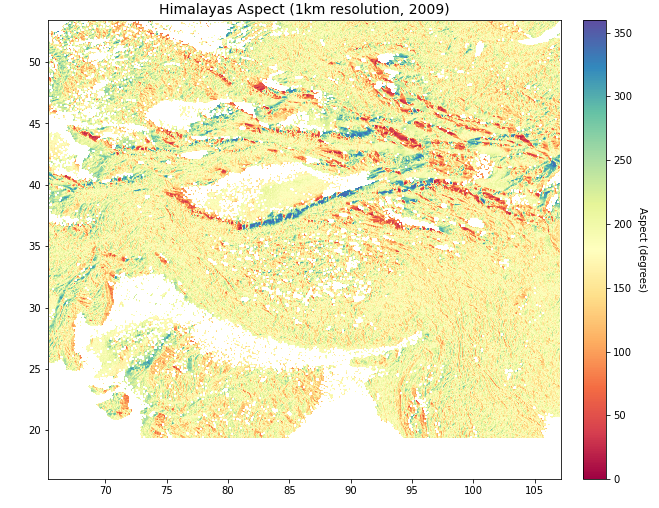
\includegraphics{./Figs/himal.png}
\end{frame}

\begin{frame}[fragile]{Ndërtojmë}
\protect\hypertarget{nduxebrtojmuxeb-3}{}
\AddToHookNext{env/Highlighting/begin}{\tiny}

\begin{Shaded}
\begin{Highlighting}[]
\CommentTok{\# llogarisim hillshade}
\NormalTok{out\_raster }\OperatorTok{=} \StringTok{\textquotesingle{}tmp/dem\_srtm\_1km\_himalayas\_2009\_hillshade.tif\textquotesingle{}}
\NormalTok{out }\OperatorTok{=}\NormalTok{ gdal.DEMProcessing(out\_raster, input\_raster, }\StringTok{\textquotesingle{}hillshade\textquotesingle{}}\NormalTok{)}
\end{Highlighting}
\end{Shaded}
\end{frame}

\begin{frame}[fragile]{Ndërtojmë}
\protect\hypertarget{nduxebrtojmuxeb-4}{}
\AddToHookNext{env/Highlighting/begin}{\tiny}

\begin{Shaded}
\begin{Highlighting}[]
\CommentTok{\# sigurohemi që skedari u shkrua}
\NormalTok{out.FlushCache()}
\CommentTok{\# out\_raster duhet të ekzistojë}
\NormalTok{hillshade\_rast }\OperatorTok{=}\NormalTok{ rasterio.}\BuiltInTok{open}\NormalTok{(out\_raster).read(}\DecValTok{1}\NormalTok{, masked}\OperatorTok{=}\VariableTok{True}\NormalTok{)}
\BuiltInTok{print}\NormalTok{(}\StringTok{"diapazoni i hillshade (në gradë):"}\NormalTok{,hillshade\_rast.}\BuiltInTok{min}\NormalTok{(),hillshade\_rast.}\BuiltInTok{max}\NormalTok{())}
\end{Highlighting}
\end{Shaded}
\end{frame}

\begin{frame}[fragile]{Ndërtojmë}
\protect\hypertarget{nduxebrtojmuxeb-5}{}
\AddToHookNext{env/Highlighting/begin}{\tiny}

\begin{Shaded}
\begin{Highlighting}[]
\NormalTok{plot\_raster(rasterio.}\BuiltInTok{open}\NormalTok{(out\_raster), hillshade\_rast, }
            \StringTok{\textquotesingle{}Himalayas Hillshade (rezolucioni 1km, 2009)\textquotesingle{}}\NormalTok{,}
            \StringTok{\textquotesingle{}Hillshade (degrees)\textquotesingle{}}\NormalTok{, cmap}\OperatorTok{=}\StringTok{"Greys"}\NormalTok{, width}\OperatorTok{=}\DecValTok{3}\NormalTok{)}
\end{Highlighting}
\end{Shaded}
\end{frame}

\begin{frame}{Ndërtojmë}
\protect\hypertarget{nduxebrtojmuxeb-6}{}
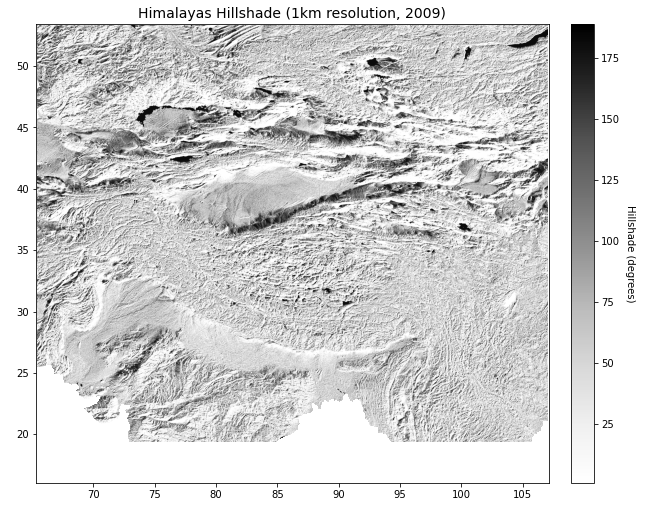
\includegraphics{./Figs/himal2.png}
\end{frame}

\end{document}
